\documentclass{llncs}
\pagestyle{headings}
\usepackage{mathtools}
\usepackage{cases}
\usepackage{multirow, booktabs}
\usepackage{algorithm}
\usepackage[noend]{algpseudocode}
\usepackage{graphicx} 
\usepackage{amsmath}
\usepackage{amsfonts}
\usepackage{xcolor}

\DeclareMathSymbol{\shortminus}{\mathbin}{AMSa}{"39}
\newcommand{\var}{\mathit{var}}
\newcommand{\VAR}{\mathit{VAR}}
\newcommand{\Pos}{\mathit{Pos}}
\newcommand{\Neg}{\mathit{Neg}}
\newcommand{\trt}[1]{\texttt{#1}}
\newcommand{\mi}{\mathit}
\newcommand{\ve}{\mathbf}
\newcommand{\btablesize}{\begin{scriptsize}}
\newcommand{\etablesize}{\end{scriptsize}}
\newcommand{\set}[2]{\{\;{#1}\;|\;{#2}\;\}}
\newcommand{\lre}{\color{red}{\{}}

\newcounter{counterName}
\allowdisplaybreaks

\begin{document}

\title{A Decomposed Fourier-Motzkin Elimination Framework to Derive Capacity Models of Container Vessels}
\titlerunning{FME for Deriving Capacity Models}
\author{Mai L. Ajspur\inst{1} \and Rune M. Jensen\inst{1} \and and Kent H. Andersen\inst{2}}
\institute{The IT University of Copenhagen \and Aarhus University}

\maketitle

\begin{abstract}
Accurate capacity models expressing the trade-off between different container types that can be stowed
on vessels are required in core liner shipping functions such as uptake-, capacity-, and network management.
Today, simple capacity models are used for these tasks, which causes overestimations. 
Though previous work on stowage planning optimization in principle provide fine-grained Vessel Stowage Models (VSMs), they are too complex to be used in the mentioned functions. 
As an alternative, this article contributes a novel framework based on Fourier-Motzkin
elimination that automatically derives Vessel Capacity Models (VCMs) from VSMs by projecting unneeded
variables. Our results show that the projected VCMs are reduced by an order of magnitude both in number of
inequalities and number of non-zero entries and can be solved up to 20-35 times faster than their corresponding VSMs with only a negligible loss in accuracy. 
Our framework is applicable to LP models in general, but are particularly effective on block-angular structured problems such as VSMs. We show similar results for a multi-commodity flow problem.
\keywords{Fourier-Motzkin Elimination \and Capacity Model \and Liner Shipping \and Projection}
\end{abstract}

\section{Introduction}
Container shipping is a central element in the clockwork of global trade \cite{EC13}. A container liner shipping company operates a set of container vessels which sail on closed loop services with fixed schedules. These services connect major trade regions like Asia and Europe, and the liner shipping business is focused on utilizing the cargo capacity in their service network. Unused capacity constitute a loss that can be fatal in a market with a profit margin of just a few percent.  
To maximize utilization of capacity, it is central for a liner shipping company to be able to estimate the residual capacity of a container vessel. This is challenging in practice, since an empty slot may be impossible to utilize for a wide range of reasons. 
For instance, the various stowage rules and seaworthiness requirements interact such that the free capacity of each container type and weight class is a complex function of the composition of cargo on board and the design of the vessel. Often it is only the stowage planning team that can determine the residual capacity of a vessel accurately, and even they may sometimes have to manually construct a stowage condition of the vessel to be able to do it. While stowage planners may be able to estimate free vessel capacity, the knowledge is primarily needed in higher order functions such as: {\em uptake management} that control the sale of cargo bookings to fill the vessels with profitable cargo; {\em capacity management} that route cargo through the service network; {\em network management} that makes changes to the service network; and {\em fleet management} that charters and buys vessels for the service network and reposition vessels between closing and opening services. Decision makers in these functions seldom have stowage insight or time to consult the stowage team. They usually boil down the free capacity of a vessel to its nominal volume, weight, and reefer (refrigerated containers) capacity minus total volume, weight and reefer number of containers already on board. This simple three dimensional capacity model is inherently optimistic, since it ignores stowage complications. It has been shown that it can lead to revenue over-estimates of more than 15\% \cite{AlbertosThesis}. This can cause sub-optimal decisions that significantly harm business.

Previous work has contributed frameworks for automated stowage planning (e.g., \cite{roach00,kimkang02,ambrosino04,low09,delgado09,pacino12}, and recently, linear stowage planning models were shown to scale to large container vessels (\cite{pacino11,AlbertosThesis}). These latter Vessel Stowage Models (VSMs) embed an accurate capacity model, but since they specify the exact positions of the containers, they are too large for use as capacity models in higher order functions, since these tasks often require several hundred capacity models to be solved simultaneously.
In this article, we present a method to calculate a Vessel Capacity Model (VCM) automatically from a linear Vessel Stowage Model (VSM).
The basic idea is to derive the VCM by abstracting away the slot position of containers in the VSM so that the model only expresses the relationship between the residual capacity of each possible container type.
Inspired by previous work in constraint programming (e.g., \cite{lassez90}) and software verification (e.g., \cite{benoy05}), we do this by projecting container position variables out of the mentioned stowage models using a framework based on Fourier-Motzkin Elimination (FME). Similar to other recent FME frameworks (e.g., \cite{simon05,lukatskii08,shapot12}), our framework includes additional features such as using equalities for substitutions (Gauss-elimination), removing syntactically redundant constraints, a complete removal of redundant constraint after each variable elimination, and a method for coarsening the boundary of the projection. Our main computational contribution is a novel decomposition method that takes advantage of block-angular structured models to significantly speed-up the projection of variables in these models. Additionally, the complete redundancy is parallellized, and the framework includes preprocessing of the constraint system including removal of less strict inequalities.

Our experimental evaluation of computing VCMs with this method shows that FME generates a large number of redundant constraints in each projection iteration that can be removed. In theory, the number of non-redundant constraints can grow exponentially with the number of projected variables \cite{monniaux10}. However, the number of constraints and non-zeros in the resulting capacity models typically are reduced by an order of magnitude compared to their corresponding stowage models. Moreover, the decomposition method reduces the size of the intermediary models produced by FME, causing less time to be needed for removing redundant constraints, which again speeds up the projection process significantly. In addition, for the models that include hydrostatic constraints, the resulting VCMs can be solved 20-35 times faster than their VSMs with only a negligible loss in accuracy. Although it can take several hours to derive a capacity model due to the clean-up of redundant constraints, this only has to be done one time for a vessel class. In this way, the approach is suitable for computing capacity models that can be applied in higher order functions of liner shipping companies such as uptake-, capacity-, fleet-, and network management. Moreover, since they are linear and much faster to solve than their corresponding stowage models, they also can be integrated in decision support systems used to optimise these functions.

Multi-commodity flow problems also have a block-angular structure, so our framework applies to these problems as well. We assume that the goal is to model how the amount of each commodity at the sinks depends on the amount of the commodities at the sources. For this purpose, the amount of each commodity that flows on edges is irrelevant and eliminated from the system. 
For this projection, we found a speed-up and a reduction in size of the resulting models similar to the ones seen for VCMs.

This paper is organized as follows. Section~\ref{sec:model} briefly present the VSMs that are projected, and Section~\ref{sec:notation} introduces the required definitions and notation. 
Then Section~\ref{sec:method} outlines the methods used in our FME framework including how block-angular problems are decomposed. 
Our experimental results then follows in Section~\ref{sec:results}. Section~\ref{sec:related} present related work, before Section~\ref{sec:conclusion} concludes.
%
%%%%%%%%%%%%%%%%%%%%%%%%%%%%%%%%%%%%%%%%%%%%%%%%%%%%%%%%%%%%%%%%%%%%%%%%%%%%%%
\section{Vessel Stowage Model}\label{sec:model}

A Vessel Stowage Model (VSM) is a set linear inequalities over continuous decision variables (i.e., a polyhedron) defining feasible stowage conditions of a container vessel. It is based on our previous work on mathematical programming models for master stowage planning [ICCL11, 12 mm]. 

Consider the container vessel shown in Figure~\ref{fig:vessel}. Each \emph{cell} on the vessel can hold two 20' containers or one 40'. Some cells have power plugs, allowing refrigerated containers (\emph{reefers}) to be stowed. Each container stack rests on sockets with maximum weight limits. Stacks are arranged longitudinal in \emph{bays} that can be further subdivided into \emph{locations}. The volume capacity of a vessel is measured in Twenty-foot Equivalent Units (TEUs) and can be more than 20K. Stowage conditions must satisfy a large number of interacting requirements. The vessel must be seaworthy with proper transversal stability and stress forces within limits. To that end, it can fill large water ballast tanks to achieve stability. The container stacks must by physically possible (e.g., 20' containers cannot be stowed on top of 40' containers) and there are separation rules for dangerous cargo. For an in-depth coverage of container vessel stowage, we refer the reader to a recent book on the topic [SSS].     
\begin{figure}[h!]
	\centering
		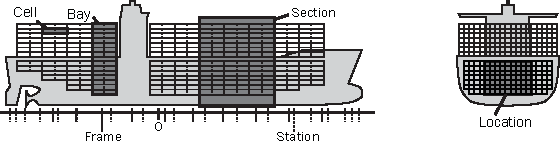
\includegraphics{figures/vessel4.pdf}
	\caption{Vessel structure and reference points.}
	\label{fig:vessel}
\end{figure}



The VSM that we investigate is based on industrial data from a large carrier that define volume, weight, and reefer capacities for each location of the vessel. Moreover, it gives positive and negative stress force limits (i.e., shear force (SF) and bending moment (BM)) for a set of \emph{frame positions}. It also contains a Bonjean table that for different drafts gives the submerged area of a cross section of the vessel for a number of \emph{station positions} (see Figure~\ref{fig:vessel}). 

The VSM considers 20' and 40' containers in three weight classes (6, 21 and 27 tons) and a container is either reefer and non-reefer. This gives total of 24 container types $T$. For each container type $\tau \in T$ and location on the vessel, there is a decision variable defining the number of containers of this type in the location. Due to the large number of containers, we ignore the integrality of these variables as previously [ICCL 11]. The VSM includes volume, weight and reefer capacity constraints for each location. To simplify the representation of hydrostatic constraints, we divide the vessel into \emph{sections} as shown in Figure~\ref{fig:vessel} and extrapolate SF and BM limits to the edge of sections. The resulting force on each section is represented by linear approximation of its buoyancy and weight. This hydrostatic modelling approach is detailed in [ICCL18]. A complete description of the VSM is given in [TEchRep]. 

A Vessel Capacity Model (VCM) is derived from a VSM by adding auxiliary variables to the VSM equal to the total of each container type and projecting all other variables out using FME. In this way the container positioning information is abstracted away. The main contribution of this paper is to introduce a novel FME framework that takes advantage of the block-angular structure of the VSM. While our experiments are carried out on the real VSM, we will for the sake of explaining the FME framework consider the simplified version shown below that mainly highlights its block-angular structure. 
\begin{numcases}{S_\texttt{g}:}
x_\tau = \sum_{i\in S} x_{i,\tau} & $\forall{\tau \in T}$\label{eq:sumT}\\
\sum_{i\in S}\sum_{\tau\in T}W_\tau x_{i,\tau} \leq D\label{eq:sumW}
\end{numcases}
\begin{numcases}{S_i\text{ for all }i\in S:} 
                                                          \smashoperator[lr]{\sum_{\tau \in T^\trt{20}}} x_{i,\tau} \leq C_i^\trt{20}                         
                                                                                                                    & $\smashoperator[lr]{\sum_{\tau \in T^\trt{20}}} W_\tau x_{i,\tau} \leq C_i^\trt{W20}$ \label{eq:cap20}\\
                                                          \;\smashoperator[lr]{\sum_{\;\tau \in T\setminus T^\trt{20}}} 2 x_{i,\tau} \leq C_i^\trt{40}
                                                                                                                    & $\smashoperator[lr]{\sum_{\tau \in T^\trt{20}}}0.5 W_\tau x_{i,\tau} + \smashoperator[lr]{\sum_{\tau \in T\setminus \in T^\trt{20}}} W_\tau  x_{i,\tau} \leq C_i^\trt{W40}$ \label{eq:cap40}\\ 
                                                                                       \smashoperator[r]{\sum_{\tau \in T^\trt{R}}} x_{i,\tau} \leq C_i^\trt{RS}
                                                                                                                    & $\smashoperator[lr]{\sum_{\tau \in T^\trt{20}}} x_{i,\tau} + 2\smashoperator[lr]{\sum_{\tau \in T\setminus T^\trt{20}}} x_{i,\tau} \leq C_i^\trt{TEU}$ \label{eq:capReefer} 
                                                                                                                   
\end{numcases}
The decision variable $x_{i,\tau} \in \mathcal{R}$ is the number containers in section $i$ of type $\tau$. There are two global constraints (\ref{eq:sumT}) and (\ref{eq:sumW}). The first defines the auxiliary variables $x_\tau$ that totals the container types (i.e., the only variables left in the VCM). The second is an assumed maximum weight $D$ of the cargo, where $W_\tau$ is the weight of type $\tau$. The following three constraints are defined for each section $i \in S$ and forms a block $S_i$ in the block-angular structure. The first and second (\ref{eq:cap20} and \ref{eq:cap40}) are volume ($C_i^\trt{20}$ and $C_i^\trt{40}$) and weight capacity ($C_i^\trt{W20}$ and $C_i^\trt{W20}$) constraints of 20' and 40' containers, respectively. Notice that the weight limits of 40' containers includes half of the weight of 20' containers due to the arrangement of sockets. The last constraint (\ref{eq:capReefer})  represents reefer ($C_i^\trt{RS}$) and total TEU capacity ($C_i^\trt{TEU}$). Notice that a 40' container counts two TEU.    






\vspace{2cm}




In this section, we will briefly introduce the vessel stowage model (VSM) that is the basis for our projections. The model is an adaption from the model presented in~\cite{ICCL18}. 
It includes various stowage constraints and further describes hydrostatic constraints reasonably accurate while
abstracting away much of the unnecessary complexity relating to the physical layout of the vessel that is present in the data describing it. 
The used data originates from a real vessel profile file used by a professional loading computer. 

\paragraph{Vessel structure and data}
The cargo space of a container vessel is divided into {bays} that each consists of a grid of {cells} that can hold two TEUs (Twenty-foot Equivalent Units), i.e. two 20' containers or one standard 40' container. Some cells have power plugs allowing for {reefer} containers to be refrigerated as required. Each bay is divided into three or four parts called \emph{locations}, at which level the vessel's capacities are given. See Figure~\ref{fig:vessel}.

On the vessel, stress forces arise as a result of gravitation acting downwards and buoyancy acting upwards. This results in shear forces and bending moments along the longitudinal axis of the vessel, and limits on these are given in the data for a set of reference points called \emph{frames}. The buoyancy force comes from the vessel's displacement of water and hence depends on the varying (and irregular) shape of the hull and the displacement of the vessel. The area submerged in water is given in the so-called bonjean table at a different set of reference points called \emph{stations} for a discrete set of displacement values. 
In general, neither frames nor stations coincide with the structures holding cargo, see Figure~\ref{fig:vessel}.


To have common reference points for cargo-holding structures and hydrostatic constraints, we define larger \emph{sections} of the vessel and use their endpoints. Each of these sections either span a number of succeeding bays, or a part of the ship containing no bays at all.
See Figure~\ref{fig:vessel}.

The weight of the empty vessel is given in the data by a set of ``blocks'' placed along the vessel with an even weight distribution.
%
The cargo itself is described by a container \emph{type}, which is defined by a length (20' or 40'), whether it is a reefer-container or not, and a weight class (in a discrete set of weights). 
Besides containers, vessels also carry \emph{ballast tanks} in fixed positions along the vessel that can be filled with water to improve the stability of the vessel.

\paragraph{Variables and constraints}
The decision variables in the VSM are the number of containers of each type $\tau$ stowed in each location $l$, and the amount of ballast water in ballast tanks in each section $s$. These are of course non-negative.
%
An important auxiliary variable is the number of containers of each type $\tau$ on the vessel in total, disregarding their placements ($x_\tau$). In the VCM, it is the relationship among these variables that we are actually interested in. Thus, when producing the VCM from the VSM, we project all variables but $x_\tau$ for all types $\tau$.  
%
\\\\
Though containers physically are placed in specific slots, the data specifies capacities for each location.
There are upper bounds for the total number of TEUs, $20'$ containers, $40'$ containers, reefer containers, reefer cells, plus {separate weight limit for $20'$ and $40'$ containers}. $20'$ containers rest on the structures midway in a cell, which $40'$s do not, leading to these two different weight limits. 
These capacity limits for each location are represented as constraints in the VSM.
%

Limits for each ballast tank are likewise given in the data, as well as a limit for the total displacement. 
Capacities for individual tanks are pooled into capacities for tanks within a section, which gives an upper bound for $t_s$. These bounds, and the bound for the total displacement are imposed as constraints in the VSM.
\\\\
In the VCM, we further have constraints that limit shear force and bending moment at the sections' end points. To obtain this from the data, we approximate the forces/moments at the sections' end points as well as the limits for these forces/moments as described below. 

First we find the area of displaced water (ADW) at a station for any displacement by linearizing the values in the discrete bonjean table. Linearizing these values, we find the ADW (for any displacement) at any given cross section of the vessel. Knowing the position of stations and the sections' end points, this gives us the volume of displaced water between each section's end points. Multiplied with $G$ (the acceleration of gravity), this is the buoyancy of the section, while the gravitational force equals the total weight of the section multiplied with $G$. Subtracting one from the other gives us the resulting force of the section. The shear force at an end point $p$ can then be calculated as the sum of resulting forces of sections fore of $p$, while the bending moment equals the sum of resulting forces of sections $s$ lying fore of $p$ times the distance from $p$ to $s$'s longitudinal midpoint.
The limit for the forces/moments at $p$ is calculated by linearizing the corresponding limits at the frame closest to $p$ at either side of it.  
A more detailed description can be found in~\cite{ICCL18} as well as a description of the accuracy of the hydrostatic approximations.

%%%%%%%%%%%%%%%%%%%%%%%%%%%%%%%%%%%%%%%%%%%%%%%%%%%%%%%%%%%%%%%%%%%%%%%%%%%%%%%%%%%%%%%%%%%%%%%%%%%%%%%%%%%%%%%%%%%%%%
\section{Definitions and notation} \label{sec:notation}
In this paper, a constraint system $S$ is a set of equalities and inequalities over the same set of variables, $\VAR(S)=\{x_1,\ldots, x_n\}$. Each constraint $c$ is either an equality, written $a_1x_1 + \ldots +a_nx_n = b$, or an inequality, written $a'_1x_1 + \ldots +a'_nx_n\leq b'$. Alternatively, we use dot-product notation for the left-hand-side, i.e. $\ve{a}\cdot \ve{x}$. 
We let $\var(c)$ denote the variables whose coefficient in $c$ is nonzero and say that $c$ \emph{uses} $x$ if $x\in \var(c)$. 
The set of points in $\mathbb{R}^{|\VAR(S)|}$ that satisfies all constraints in $S$ is called $S$'s \emph{feasible area}. A constraint $c\in S$ is \emph{redundant} iff it does not influence the feasible area for $S$, otherwise it is called \emph{non-redundant}.  

For some variables $Y\subseteq \VAR(S)$, we are not interested in their values in a feasible point - we just want to know that a satisfying value exists. This property is captured by the \emph{projection of $S$ w.r.t. $Y$}, which is the largest set consisting of values for $\VAR(S)\setminus Y$ that can be extended with values for $Y$ such that all constraints in $S$ are satisfied. 
%
The projection of a constraint system is a uniquely determined subset of $\mathbb{R}^{|\VAR(S)\setminus Y|}$, but also the feasible region of another system $S'$ (see e.g. \cite{ziegler95}). We are mostly interested in the latter, since it is the relationship between the values in the projection that is relevant to us, and we allow ourselves to write that ``$S'$ is the projection of $S$ w.r.t. $Y$'' if the feasible area of $S'$ equals the projection of $S$, though such a system is not uniquely determined.
We note, that since we are dealing with subsets of multi-dimensional Euclidian spaces, the dimension and the order of the variables are important. However, in order to simplify the presentation, we do not explicitly specify these for every considered projection/constraint system $S'$. A more stringent exposition keeping track of the variable sets and ordering can be found in \cite{MyTechRep}.
%%%%%%%%%%%%%%%%%%%%%%%%%%%%%%%%%%%%%%%%%%%%%%%%%%%%%%%%%%%%%%%%%%%%%%%%%%%%%%%%%%%%%%%%%%%%%%%%%%%%%%%%%%%%%%%%%%%%%%
\section{Solution method} \label{sec:method}
This section introduces our FME-based projection framework for calculating the projection of the constraint system $S$ w.r.t. $Y$. It can be used for massive variable elimination in any linear inequality system but has been designed to take advantage of block-angular structures often found in real-world models including the VSM. 
The methods for projecting any (not necessarily structured) constraint system are described in Section~\ref{sec:projMethod}, while the decomposition used on block-angular structured problems will be described in Section~\ref{sec:decomp}.

\subsection{Projection procedure}\label{sec:projMethod}
The projection procedure starts with a preprocessing of the constraint system, i.e. we reduce it by removing easily identifiable redundant constraints and assign necessary bounds and values to variables (e.g., \cite{brearley75,andersen95,maros}).
Then we use the equalities in the reduced system to isolate variables from $Y$ and substitute in the rest of the system, %. This eliminates variables from the system, and we 
referred to as \emph{Gauss-elimination} (e.g., \cite{duffin74,simon05}).  
Subsequently, we successively eliminate one variable from $Y$ using Fourier-Motzkin elimination and remove redundant inequalities from the system afterwards, until no more variables remain to be eliminated. Eliminating a variable from the system causes some of its constraints to be removed, while new inequalities are added. Only the added inequalities are checked for redundancy. % since the remaining constraints have already have been checked previously and do not later become redundant. 
At the top-level, the pseudocode for our projection method is thus as described in the pseudocode in Algorithm~\ref{alg:FMEF}. 
\setlength{\floatsep}{10pt} %standard minimum er vist 16
\setlength{\textfloatsep}{14pt} %standard minimum er vist 16
\begin{algorithm}[tb]
\caption{Projection based on Fourier-Motzkin elimination} 
\label{alg:FMEF}
\begin{algorithmic}
\Function{Project}{System $S$, Variables $Y$}
	\State $(S,Y)\gets \Call{Preprocess}{S,Y}$
	\State $(S,Y)\gets\Call{Gauss-Elim}{S,Y}$
	\While{$Y\neq\emptyset$}
		\State $(S, Y, New )\gets\Call{FME-SingleVar}{S,Y}$
		\State $S\gets\Call{RemoveRedundancy}{S,New}$
	\EndWhile
	\State \Return $S$
\EndFunction
\end{algorithmic}
\end{algorithm}
Each sub-procedure in this algorithm is detailed further below. We start with the methods for variable elimination, before we describe the redundancy removal and finally the preprocessing step. 

\paragraph{Fourier-Motzkin-elimination} 
Fourier-Motzkin Elimination (FME) is a classical algorithm for producing the projection of a set of variables from an inequality system, i.e. a constraint system with no equalities. The method successively eliminates one variable $x\in Y$ until all required variables have been eliminated. To eliminate $x\in Y$, the constraints in $S$ are first divided into sets, $\Pos_S(x)$, $\Neg_S(x)$, and $\mi{Zero}_S(x)$ depending on the sign of $x$'s coefficient. 
Each equality is treated as two inequalities, and bounds are treated as any other inequalities. 
A new system $S'$ is then created, which is the projection of $S$ w.r.t. $\{x\}$. It consists of $\mi{Zero}_S(x)$, together with one inequality, $i_{p,n,x}$, for each pair $(p,n)\in \Pos_S(x)\times \Neg_S(x)$. $i_{p,n,x}$ is the addition of positive multiples of $p:\ve{a}\cdot\ve{x} \leq b$ and $n:\ve{a}'\cdot\ve{x} \leq b'$ such that the coefficient of $x$ in the resulting inequality is $0$, i.e.
\[
i_{p,n,x}: -a'_x\cdot \ve{a}\cdot\ve{x} + a_x\cdot \ve{a}'\cdot\ve{x} \leq -a'_x\cdot b + a_x\cdot b'.
\]
The order in which variables are eliminated naturally influences the size of the intermediary inequality systems. We have chosen to use the greedy heuristic {that minimizes the number of new inequalities in the immediately next system \cite{duffin74}}, which is a commonly used heuristic. It is easily calculated from the current system as the variable $x\in Y$ that minimizes $|\Pos_S(x)||\Neg_S(x)| - |\Pos_S(x)|-|\Neg_S(x)|$.  In the worst case scenario, %where $|\Pos_S(x)| = |\Neg_S(x)| = \frac{|S|}{2}$ for all $x\in Y$, 
the number of inequalities in the created system $S'$ is $\frac{1}{4}|S|^2$, which implies that (both time and space) complexity is double-exponential. For a large, dense system, the growth will be substantial, which prohibits it from use for practical purposes \emph{if} the added inequalities are non-redundant or the non-redundant inequalities are not removed ({see e.g. \cite{lassez93} and \cite{lukatskii08}}). It should, however, also be emphasized that not all inequalities in the succeeding system are necessarily non-redundant; in fact, the number of non-redundant inequalities will at most grow exponentially \cite{monniaux10}.

\paragraph{Gauss-elimination} 
An equality $e$ can be used to isolate a variable $x\in Y$ which can then be substituted in all other constraints in $S$ (a Gauss-elimination). This eliminates $x$ from the system and does not cause the same combinatorial explosion of inequalities as FME may do (e.g., \cite{duffin74,simon05}). Before performing FME we therefore do as many Gauss-elimination of variables in $Y$ as possible. To avoid density, when the system $S$ contains several equalities, we first choose the variable $x$ (used in any equality) that is used the fewest times in total in $S$. We then choose the equation $e$ among those using $x$ that uses the fewest variables, and do Gauss-elimination of $x$ using $e$. This is then repeated until there are no more equalities using variables from $Y$.

\paragraph{Redundancy removal} 
To detect redundancy, we examine each inequality $c: \ve{a}\cdot \ve{x}\leq b$ in turn and remove it from the system if $\max \ve{a}\cdot \ve{x}$ subject to $S\setminus\{c\}$ is less than or equal to $b$. The property can be checked using an LP solver. Only \underline{in}equalities are examined, since we want to keep the equalities for use in Gauss-elimination. Not all inequalities have to be examined, though. When removing redundancy after projecting $x$ from $S$ we do not need to check inequalities in $\mi{Zero}_S(x)$; if they were non-redundant before the elimination, they will be non-redundant after.

For large systems, checking all constraints for redundancy is time-consuming. We have therefore implemented a method for redundancy removal that uses several threads in parallel. Each thread checks one inequality at a time, while a manager takes care of the communication and keeps track of the found redundant inequalities. 
For the method to work correctly, it is important that $S$ contains no two constraints defining the same halfspace since each one on its own would be redundant due to the other. Such easily detectable redundancies are removed prior to the redundancy removal. We notice that rational numbers are used in the implementation to avid rounding errors. 

Several of the constants in the data used for our vessel models are results of various approximations and hence the boundary of the feasible area is not exact. Coarsening the boundary is therefore permissible, and we also remove inequalities that are \emph{``almost redundant''}. An inequality $c: \ve{a}\cdot\ve{x}\leq b$ is almost redundant if $\max \ve{a}\cdot\ve{x}$ subject to $S\setminus\{c\}$ is less or equal to $b + \epsilon\cdot |b|$ for a small $\epsilon$, see Figure~\ref{fig:almostRedundant}; for our experiments we have used $\epsilon = 0.02$. If $b=0$, we instead require the maximum to be smaller than a given $\epsilon'$. 
\begin{figure}[tb]
	\centering
		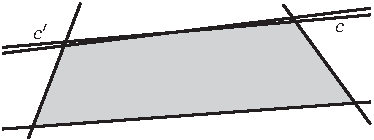
\includegraphics[scale=0.7]{figures/almostRedundant2.pdf}
	\caption{The inequality $c$ is almost redundant compared to $c'$, and vice versa.}
	\label{fig:almostRedundant}
\end{figure}
Therefore, the manager also collects a set of almost redundant inequalities; the property is checked simultaneously with the ordinary redundancy check. After the parallel redundancy check, \emph{one} thread is then used to go through all the almost redundant inequalities one by one, and the ones that are still almost redundant are removed. 
%
This \emph{cannot} be done in parallel. Otherwise, both $c$ and $c'$ in Figure~\ref{fig:almostRedundant} could be found almost redundant by two different threads, causing them both to be eliminated. In a sequential check, however, only the first to be examined would be removed. 

Methods for coarsening the boundary of the feasible area that relies on removing almost redundant inequalities are also used in \cite{lukatskii08} and \cite{shapot12}, though their approaches are different.

\paragraph{Preprocessing}
Prior to the projection, we perform some simple preprocessing steps repeatedly as long as a reduction happens. For this, we maintain an upper and lower bound for each variable and each constraint's left-hand-side. 
The bounds of a constraint is linked to the bounds of the variables it uses, so tightening a bound of a variable or constraint can imply a tightening of another bound. 

The steps are implemented with special care of equalities and working with the assumption that the system is feasible (details can be found in \cite{MyTechRep}).
Besides updating bounds, we remove all empty inequalities and unused variables $x\in Y$.  
%
If the upper and lower bounds of a constraint (or variable) are equal, each of the used variables are substituted with its upper or lower bound that results in the constraint's bound. 

%
We remove a constraint $\ve{a}\cdot \ve{x} \leq b$ if its upper bound 
is less or equal to $b$. 
If the same is true for an equality $\ve{a}\cdot \ve{x}=b$, due to the feasibility assumption, the variables used in $c$ are substituted with the bounds that makes $\ve{a}\cdot \ve{x}$ equal $b$. 


If $\Neg_S(x)=\emptyset$ for an $x\in Y$ 
then we remove all constraints in $\Pos_S(x)$. If $\Neg_S(x)$ only consist of the inequality defining the lower bound of $x$, $-x\leq -lb_x$, then we substitute $x$ with $lb_x$ in all constraints. Similarly w.r.t. $\Pos_S(x)$. We notice that this is \emph{not} a normal preprocessing step, but corresponds to making a FME on $x$, and this changes the feasible area of $S$. 

Comparing two constraints $c$ and $c'$ syntactically, we can in some cases detect redundancy. 
If $c:\ve{a}\cdot \ve{x}\otimes b$ and $c': \ve{a}'\cdot \ve{x}\otimes' b'$ (where $\otimes,\otimes'\in\{\leq,=\}$), the following holds.
\begin{itemize} \itemsep0em 
\setcounter{enumi}{\value{counterName}}
\item 
If $\ve{a}=\sigma\cdot \ve{a}'$, then $c$ and $c'$ are \emph{linearly dependent} (\cite{lassez93}). Hence, $c$ is redundant if
it is an \underline{in}equality and $\sigma\cdot b'\leq b$ and either: $\sigma\geq 0$; or $\sigma<0$ and $c'$ is an equality. $c$ is also redundant if both $c$ and $c'$ are equalities and $\sigma\cdot b'\leq b$. 
\item
If all variables used in $c$ and $c'$ are non-negative, and there exists a $\sigma\geq 0$ such that $a_x \leq \sigma \cdot a'_x$ for all $x$, while $\sigma\cdot b' \leq b$, then $c$ is \emph{less strict} than $c'$; it is redundant and hence removed. If $c$ is an equality, so must $c'$ be, and hence $c'$ is turned into an equality. 
\end{itemize} 
%%%%%%%%%%%%%%%%%%%%%%%%%%%%%%%%%%%%%%%%%%%%%%%%%%%%%%%%%%%%%%%%%
\subsection{Decomposing block-angular structured system}\label{sec:decomp}
In the following we will describe how the block-angular structure of a system can be exploited to make our projection framework scale. Detailed pseudocode and correctness proofs can be found in \cite{MyTechRep}. 

The constraints defining the capacity for a section $i$ can be collected in a \emph{local} subsystem $S_i$, whose constraints only use variables that are not used in $S_{i'}$ for another section $i'$. The remaining constraints make up another \emph{global} subsystem, $S_\texttt{g}$, where the constraints also use variables from several of the local subsystems. That is, the constraints in the VSM have a natural \emph{(primal) block-angular structure} \cite{williams} as depicted in Figure~\ref{fig:decomp2}.

To obtain a VCM, we want to eliminate all but the variables counting the total number of containers of each type. The variable being eliminated is (with high probability) used in the global constraints, which causes the inequalities constructed by FME to use variables from all subsystems, that is, the local subsystems gets ``mixed''. This result in an increasing number of global and more dense constraints, which again makes FME perform worse. 
To avoid the immediate mix of variables, we will define and use auxiliary variables to ensure that we can project the local subsystems separately without producing global constraints, before we combine the projected subsystems and eliminate the auxiliary variables. To separate and remove local variables from the global constraints, we do as follows for all subsystems $S_i$.

\begin{itemize}\itemsep0em
\item For each global constraint $c$ using variables in $S_i$, we define an auxiliary variable $z^0_{c,i}$ that equals the variables in $S_i$'s contribution to $c$. We add the equality defining $z^0_{c,i}$ to $S_i$, and we substitute with it in $c$. 
We name the thusly produced subsystem $S_i^0$. 
\item Then, we project $S_i^0$ w.r.t. all variables from $Y\cap X_i$, where $X_i=\mi{var}(S_i)$, resulting in the system $S'^{\,0}_i$. We do keep the auxiliary $z^0$-variables. 
Because of these auxiliary variables this only produces inequalities with variables not present in other subsystems $S_j$. 
\end{itemize}
After projecting each $S_i^0$ we can then combine the results with the rephrased, global constraints, $S_\trt{g}^0$, to create the system $\mathcal{S} \overset{\text{def.}}{=}
\mathcal{S} = S^0_\trt{g} \cup S'^{\,0}_1\cup \ldots \cup S'^{\,0}_k$.
We can then eliminate from $\mathcal{S}$ all the auxiliary $z^0$-variables, $Z^0$, plus any remaining variables in $Y$. 

\paragraph{Example}
As an example, we consider an extremely simplified VSM consisting of the constraints indicating the capacities for each section $i\in S$, constraints that counts the total of each type $\tau\in T$, and a constraint that limits the total weight of cargo. That is, the constraint system is:
\begin{align*}
S_i \text{ for all }i\in S&: \left\{ \begin{array}{ll}
		\smashoperator[r]{\sum_{\tau \in T^\trt{20}}} x_{i,\tau} \leq C_i^\trt{20} 									& \quad\smashoperator[r]{\sum_{\tau \in T^\trt{20}}} W_\tau\cdot x_{l,\tau} \leq C_l^\trt{W20}\\
		\smashoperator[r]{\sum_{\tau \in T\setminus T^\trt{20}}} 2\cdot x_{i,\tau} \leq C_l^\trt{40}& \quad 0.5 \smashoperator[lr]{\sum_{\tau \in T^\trt{20}}} W_\tau\cdot x_{l,\tau} + \smashoperator[lr]{\sum_{\tau \in T\setminus \in T^\trt{20}}} W_\tau\cdot x_{l,\tau} \leq C_l^\trt{W40} \\
		\smashoperator[r]{\sum_{\tau \in T^\trt{R}}} x_{l,\tau} \leq C_l^\trt{RS}										& \quad \smashoperator[lr]{\sum_{\tau \in T^\trt{R}\cap T^\trt{20}}} 0.5\cdot x_{l,\tau} + \smashoperator[lr]{\sum_{\tau \in T^\trt{R}\setminus T^\trt{20}}} x_{l,\tau} \leq C_l^\trt{RC}\\ 
		&\quad \smashoperator[r]{\sum_{\tau \in T^\trt{20}}} x_{l,\tau} + 2\cdot\smashoperator[lr]{\sum_{\tau \in T\setminus T^\trt{20}}} x_{l,\tau} \leq C_l^\trt{TEU}
\end{array}\right.\\
S_\texttt{g} &: \left\{ \begin{array}{ll} 
			x_\tau = \sum_{i\in S} x_{i,\tau} & \forall{\tau \in T}\\		
			\sum_{i\in S}\sum_{\tau\in T}W^\tau x_{i,\tau} \leq D
\end{array}\right.
\end{align*}
This is naturally block-angular structured since each $S_i$ constitutes a local system, while the remaining constraints, $S_\texttt{g}$, makes up the global constraints.  

To obtain a less detailed VCM from this VSM, we want to eliminate all variables but $\set{x^\tau}{\tau\in T}$. 
To exploit the structure of the system, we first define a variable to hold the weight of cargo in each section $i$, $w_i$. We also define the variable $x'_{i,\tau} = x_{i,\tau}$, although this is only a renaming of the variables at first glance. We add the defining constraints to the relevant local system, and redefine the global constraints in terms of the new variables. 
That is, the $i$'th local subsystem is now $S_i^0 = S_i \cup \{w_i = \sum_{\tau\in T} W^\tau x_{\tau,i}\} \cup \bigcup_{\tau\in T}\{x'_{i,\tau} = x_{i,\tau}\}$, while the new system of global constraints is $S_g^0 = \cup_{\tau\in T}\{x^\tau = \sum_{i\in S} x'_{i,\tau}\} \cup \{w_1 + w_2 + w_3 + w_4 \leq D\}$. 

Notice, that due to the new auxiliary variables, for a given $i\in S$, none of the variables $x_{i,\tau}$ is used in any constraints outside of $S^0_i$. Therefore, to project $\set{x_{i,\tau}}{\tau\in T}$ from the whole system ($S^0_g\cup_{i'\in S}S^0_{i'}$) we can just eliminate $\set{x_{i,\tau}}{\tau\in T}$ from $S_i^0$ (that is, we keep $\{x_{\tau,i}, w_i\}$), and then add the projection to the other subsystems and the global constraints. And then we can do that for the other subsystems. 
In the end, when all subsystems $S^0_i$ have been projected, we can join these projections together with $S^0_\trt{g}$ and eliminate the remaining variables, $\set{x'_{i,\tau}}{\tau\in T, i\in S}\cup\set{w_i}{i\in S}$ from this.
\\\\
\noindent Comparing $\mathfrak{S} \overset{\text{def.}}{=} S_1^0\cup\ldots\cup S_k^0\cup S_\trt{g}^0$ with the original system $S$, all we have done is defining auxiliary variables and substituted them in the system. Thus, eliminating $Y$ from $S$ is equivalent to eliminating $Y \cup Z^0$ from $\mathfrak{S}$. 
%
When eliminating $Y\cup Z^0$ from $\mathfrak{S}$, we can choose to first eliminate $X_1\cap Y$, then $X_2\cap Y$ up to $X_k\cap Y$, and finally $Z^0\cup Y\setminus(X_1\cup \ldots\cup X_k)$. 
Any variable in $X_1\cap Y$ has a zero-coefficient in all constraints outside $S^0_1$, so $\mathfrak{S}\setminus S^0_1$ will not be changed by FME when $X_1\cap Y$ is eliminated. It can therefore be put aside until that projection is done. 
Likewise, when eliminating $X_i\cap Y$, neither $S_{i+1}^0\cup \ldots \cup S_k^0\cup S_\trt{g}^0$ nor the already projected systems contain any variables from $X_i\cap Y$ and can hence be put aside until the variables in $Z^0\cup Y\setminus(X_1\cup \ldots\cup X_k)$ are eliminated. Thus, the following holds. 
%
\begin{proposition}
The projection of $S$ w.r.t. $Y$ defines the same feasible area as 
the projection of $\mathcal{S}$ w.r.t. $Z^0 \cup Y\setminus (X_1\cup \ldots \cup X_k)$. 
\end{proposition}
%
$\mathcal{S}$ has by construction a block-angular structure and instead of eliminating $Z^0\cup Y\setminus(X_1\cup\ldots\cup X_k)$ immediately, if necessary, we can use the same approach as above to postpone ``mixing'' blocks.
To do so, we collect all subsystems into $k_1$ small groups and do the following for each group $i$: 
\begin{itemize}\itemsep0em
\item We join the systems in the group into a new system, $S^1_i$. For each (rephrased) global inequality $c$ using variables occurring in $S^1_i$, we then define a variable, $z^1_{c,i}$, that equals $S^1_i$'s contribution to $c$. We add the defining equality to $S^1_i$ and rephrase $c$ using $z^1_{c,i}$.
\item Then we project the resulting system, $S^1_i$, w.r.t. the previous, auxiliary $z^0$-variables, while we keep the newly created $z^1$-variables.
\end{itemize} 
Subsequently we can then join the projected $S^1$-systems with $S_\trt{g}^1$, and finally project the last auxiliary variables. Alternatively, we can repeat the steps above until the final projection can be done. 

When we decompose a system as described above, we effectively create a tree structure of subsystem paired with a set of variables to be eliminated. An inequality system can then be projected by recursively projecting its children. See Figure~\ref{fig:decomp2} and the example further below.

\begin{figure}[tb]
	\centering
		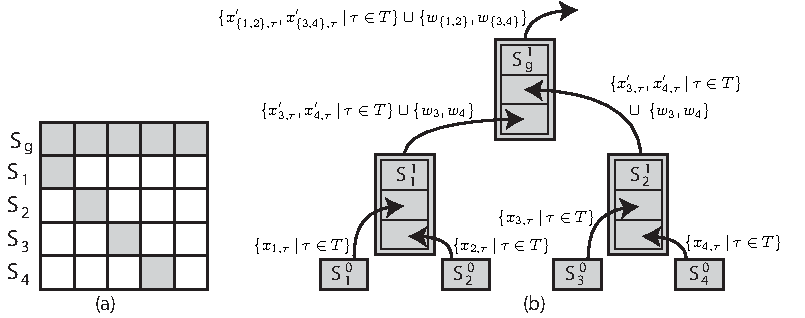
\includegraphics[scale=0.9]{figures/Example5.pdf}
	\caption{(a) A block-angular structured system. (b) Projection using tree-structure.}
	\label{fig:decomp2}
\end{figure}

The intuition why this works is as before; projecting all $Y$ and $Z$-variables from the union of all the (unprojected) subsystems in the nodes of the tree corresponds to projecting the $Y$ variables from $S$, and because we can choose the elimination order of the variables, we only need to project the subsystems in the tree in the correct order (a rigorous proof can be found in \cite{MyTechRep}).

\begin{proposition}
The projection of the system associated with the root of the tree constructed from $S$ and $Y$ w.r.t. the $Y$- and $Z$-variables as described corresponds to projecting $S$ w.r.t. $Y$.
\end{proposition}

\paragraph{Example}
Consider the system from the previous example, which was decomposed into the subsystems $S^0_\trt{g}$ and $S^0_i$ for $i\in S$. Instead of projecting these subsystems as described in the previous example, if for examples the constraints in $S^0_\texttt{g}$ uses too many variables, we can insert an additional level in the decomposition. 
Assume for instance that $S=\{1,2,3,4\}$. Then we can group the four subsystems into two groups, $\{S^0_1, S^0_2\}$ and $\{S^0_3, S^0_4\}$, and for each global constraint, we define a variable stating each new group's contribution to the global constraint. For example, we define a variable $w_{\{1,2\}}$ that is the weight of the containers in section 1 and 2. The defining variables are added as a new subsystem, and the global constraints are rephrased. That is, we construct the subsystems %I.e. we construct the tree structure in Figure~\ref{fig:decomp2}(a), where 
\footnotesize{
\[
\begin{gathered}
S_\trt{g}^1 :\{ x^\tau = x'_{\{1,2\}} + x'_{\{3,4\}},\: w_{\{1,2\}} + w_{\{3,4\}} \leq D \},\\   
S^1_1				:\{ x'_{\{1,2\}} = x'_{1} + x'_{2},\: w_{\{1,2\}} = w_{1} + w_{2}\},\:
S^1_2				:\{ x'_{\{3,4\}} = x'_{3} + x'_{4},\: w_{\{3,4\}} = w_{3} + w_{4}\}. 
\end{gathered}
\]}
\normalsize{These systems compose a tree structure, whose root is projected recursively as shown in Figure~\ref{fig:decomp2}(b) to obtain the projection of the original VSM.}
\\\\
Using our previously described projection method, we obtain the projection of $S$ w.r.t. $Y$ by calling \Call{ProjectNode}{root of $T$}, where $T$ is the tree structure constructed from $S$ and $Y$, and \Call{ProjectNode}{} is described in Algorithm~\ref{alg:decomp}. We note that due to the elimination of almost redundant inequalities, this only approximates the projection. However, by setting $\epsilon = 0$, the algorithm indeed returns the correct projection.

\begin{algorithm}[tb]
\caption{{Projecting a block-structured system via decomposition.}}
\label{alg:decomp}
\begin{algorithmic}
\Function{ProjectNode}{Node $n$} 
	\State $(S,Y)\gets$ the system and variable set associated with $n$
	\If{$n$ is a leaf}
		\State \Return \Call{Project}{$S$, $Y$}\Comment Algorithm~\ref{alg:FMEF}
	\Else
		\ForAll{children $m$ of $n$}
			\State $S \gets S\cup \Call{ProjectNode}{m}$ 
		\EndFor
		\State \Return $\Call{Project}{S, Y}$ \Comment Algorithm~\ref{alg:FMEF}
	\EndIf
\EndFunction
\end{algorithmic}
\end{algorithm}
%
\noindent Using the described decomposition, it is of course also possible to project nested block structured problems, i.e. systems that on the top-level can be divided into a global part and a number of local parts that in themselves can be further divided into local parts and a global part, and so on.  
Other block structured problems such as staircase problems can also be decomposed into a tree structure and projected using the described approach. 
%\paragraph{\red{Parallelization}}

Further, when the system $S$ is decomposed into subsystems in a tree structure, the projection itself can be parallelized by maintaining a queue of not yet projected subsystems whose children have all been projected; this queue thus initially contains all leafs. 
The members of the queue are then solved independently by multiple solvers in parallel, who also add systems to the queue when the membership condition is met.
%The pseudocode for this is presented below. Besides a system $S$ and a variable set $Y$, each node $n$ is associated with a number, $n_{count}$, corresponding to the number of projected children (initially set to $0$), and a system, $n_{proj}$, corresponding to the projection $\mi{proj}_Y(S)$ when it is done (initially set to $\emptyset$). 
%\vspace{1mm}
%
%\begin{algorithmic}
%\Function{ParallelTreeProjection}{$S$, $Y$}
%	\State Construct  tree structure $T$ from $S$ and $Y$
%	\State $n_{count}\gets 0$ and $n_{proj}\gets\emptyset$ for all nodes $n$ in $T$
%	\State Create a set $W$ of workers, initially idle
%	\State Initialize a queue $Q$ with all leaves in $T$
%	\While{$\mi{root}(T)_{proj} = \emptyset$}
%		\If{$Q$ is non-empty and a worker $w\in W$ is idle}
%			\State Remove first node $n$ from $Q$
%			\State Use $w$ to call \Call{ProjectSingleNode}{$n$}
%		\EndIf
%	\EndWhile
%	\State \Return $\mi{root}(T)_{proj}$
%\EndFunction
%\Statex
%\Function{ProjectSingleNode}{Node $n$}
%	\State $(S',Y')\gets$ the system and the variable set associated with $n$
%	\State $S'\gets S'\cup_{m\in \mi{children}(n)} m_{proj}$ 
%	\State $n_{proj}\gets$ \Call{Project}{$S'$,$Y'$} \Comment Algorithm~\ref{alg:FMEF}
%	\State $\mi{parent}(n)_{count} \gets \mi{parent}(n)_{count} +1$
%	\If{$\mi{parent}(n)_{count} = |\mi{children}(\mi{parent}(n))|$}
%		\State Add $\mi{parent}(n)$ to $Q$
%	\EndIf
%	\State \Return
%\EndFunction
%\end{algorithmic}	
%
%\vspace{1mm}
Since all parallel workers project a system using the FME framework, which again involves parallel redundancy removal, it is important to only use as many resources (threads) in total as there are available.
%Then, when at some point there are less nodes left to project than there are workers in $W$, the superfluous workers can pass on their resources to the remaining workers.  

%%%%%%%%%%%%%%%%%%%%%%%%%%%%%%%%%%%%%%%%%%%%%%%%%%%%%
\section{Results}\label{sec:results}
We have constructed a number of different VSMs from data for a specific vessel, where the weight and hydrostatics are taken into account to various degrees. The first VSM has no limit on the total displacement or any hydrostatic constraints, the second VSM does not model any hydrostatic constraints, and the subsequent VSMs (refered to as complex VSMs) consider the hydrostatic constraints at 2, 4, 6 and 8 measure points, respectively. 
Each VSM has been transformed into its corresponding VCM by eliminating all variables except the $x_\tau$ variables. Projections have been done in two different ways, \emph{decomposed} and \emph{flat}. For the decomposed projections, a tree structure has been used as described previously, while the flat projections do not use any decomposition at all. 

The VSMs and VCMs have been optimized for revenue. The optimal objective value as well as time taken has been compared. The latter is measured in both iterations and \emph{ticks} as it appears when solved with CPLEX Interactive Optimizer version 12.5.0.0. Ticks is a deterministic time measure that according to the software provider ``yields the same level of performance for repeated solving of the same model with the same parameter settings, on the same computing platform''. The revenue is dependent on the container type, so that the container types that (in the industry) are found more limiting also yields a higher revenue, see further below. 

Our FME-based projection framework has been implemented in Java. The experiments were carried out on a computer with an {Intel\textsuperscript{\textregistered} Xeon\textsuperscript{\textregistered} E5-1660 V4 processor with a frequency of 3.20-3.80 GHz, 32GB RAM, and with 8 cores and 16 threads.}

\paragraph{Size reduction}
Table~\ref{tab:projections} summarizes the size of the VSMs and the VCMs that are the result of the projection using decomposition. These sizes are given in terms of the number of inequalities (ineq), equalities (eq), variables (var), non-zero entries (nzs) and density (dens). The size of the VSMs are given both as they appear as input to our algorithm, but also after it has been preprocessed by CPLEX. For comparison, the table includes the simple VCM for the vessel in question, which is the one currently used in the industry. %, and it only includes upper bounds on the total number of containers, the total number of reefer containers, and the total weight.  

\begin{table}[tb]
\caption{The size of the VSMs and corresponding VCMs.}
\label{tab:projections}
\centering
\btablesize
\begin{tabular}{l|*{2}{*{3}{r@{\:\;}}r|}*{3}{r@{\:\;}}r}
$\multirow{2}{*}{}$&\multicolumn{4}{c|}{VSM}&\multicolumn{4}{c|}{VSM, presolved}& \multicolumn{4}{c}{VCM}\\
							&ineq (eq)&var &nzs & dens  &ineq &var	&nzs	&dens&ineq &var &nzs &dens\\
\hline
{No weights}	&774 (12)	&1142&6662&8.61		&554	&657	&2784	&5.03&	20 &12	& 155&7.75\\   %554/20 = 27,7, 657/12 = 54,74,  2785/155 = 17,97
{No hydro.} 	&806 (43)	&1173&7854&9.74		&555	&657	&3441	&6.20&	18 &12	& 144&8.00 \\  %555/18 = 20,8, same							3441/144 = 23,89
{2 parts} 		&810 (43)	&1173&7860&9.70		&556	&661	&3447	&6.20&	96 &12	&1113&11.59\\  %556/96 = 5,8, 661/12 = 55				3447/1113 = 3,09
{4 parts} 		&824 (49)	&1179&7886&9.57		&564	&671	&3471	&6.15&	64 &12	& 731&11.42\\  %564/64 = 8,8										3471/731 = 4,74
{6 parts} 		&838 (55)	&1185&7916&9.44		&570	&679	&3496	&6.13&	80 &12	& 888&11.10\\  %570/80 = 7,1										3496/888 = 3,94
{8 parts} 		&852 (61)	&1191&7950&9.33		&576	&685	&3522	&6.11&	52 &12	& 582&11.19\\  %576/52 = 11,1 685/12 = 57.1			3522/582 = 6,05
\bottomrule
Simple VCM 		& 3\phantom{ (55)}&12 &\phantom{12}36&12.00&3&9&\phantom{12}24&\multicolumn{1}{l}{8.00}\\
\end{tabular}
\etablesize
\end{table}
Since we project all but 12 variables, this naturally gives a large reduction in the number of variables, more precisely 54-57 times fewer than even the presolved VSMs. However, the VCMs also have 5.8-11.8 times fewer inequalities than the presolved VSMs (for complex VSMs) while they two others have 20.8-27.7 times fewer constraints. The VCMs also have fewer non-zero entries (3-6 times fewer for complex VSMs, and otherwise 18-24). The results reveal no apparent relationship between the size of the VSM and the size of its VCM. This may be due the actual position of the hydrostatic measure points as well as the non-deterministic behaviour of the removal of almost redundant inequalities. 

\paragraph{Decomposition impact}
Table~\ref{tab:time} shows the time taken for the algorithm to do the projection, both decomposed and flat. For most VSMs, the flat projection timed out (TO) (the computations were stopped after 18-65 hours), in which case the variables left to be projected are given. Figure~\ref{fig:8parts}(a) shows the progression of the number of inequalities and variables, respectively, as a function of time when the algorithm runs on the decomposed 8 part model. These numbers are the sum of all the inequalities and variables, respectively, in all the projected or unprojected subsystems in the decomposition at a given time. Likewise, Figure~\ref{fig:8parts}(b) shows the progression for the flat projection of the same model; this figure includes the number of inequalities for the decomposed projection for comparison. Each graph shows the number of inequalities and variables after each step outlines in Section~\ref{sec:projMethod}. %preprocessing step, each Gauss-elimination, and each FM-elimination followed by some preprocessing, parallel redundancy removal and sequential removal of almost redundant inequalities.    
\begin{table}[tb]
\caption{Projections time.}
\label{tab:time}
\centering
\btablesize
\begin{tabular}{l|r@{\hspace{0em}}rc|rc}
&\multicolumn{3}{c|}{Decomposed}&\multicolumn{2}{c}{Flat}\\
&\multicolumn{2}{c}{time}& vars left &\multicolumn{1}{c}{time}&vars left\\
\hline
{No weights}& &24.5m&-&2.5m&-\\
{No hydro.}& &14.5m&-&1.8m&-\\
{2 parts} &7h&18m &-&(TO) 32h& 551\\
{4 parts} &8h&4m &-&(TO) 61h & 557\\
{6 parts} &3h&7m &-&(TO) 18h & 577\\
{8 parts} &3h&19m &-&(TO) 65h& 566\\
\end{tabular}
\etablesize
\end{table}

The results in Table~\ref{tab:time} shows that the decomposition has a substantial impact on the success of the projection of the complex VSMs. However, the two non-complex VSMs are solved faster using a flat projection. This behaviour is not surprising, since the hydrostatic constraints are dense, global constraints that links the weight of all sections to the left or right of a measure point, and the coefficients in the constraints are non-trivial. Thus, when these are included, decomposition is useful while not necessary for the simpler systems.
 
\begin{figure}[tb]
	\centering
		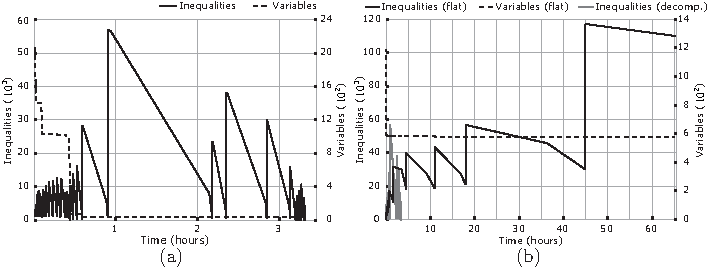
\includegraphics{figures/newDecompFig.pdf}
	\caption{The inequalities growth and variable decrease for the 8 part-model (a) with decomposition and (b) flat.}
	\label{fig:8parts}
\end{figure}

When considering each subsystem in a decomposition as a system in itself, in general, the number of inequalities after each call to \Call{FME-SingleVar}{} in Algorithm~\ref{alg:FMEF} grows to begin with, as does the number of inequalities before this call. This continues until there are a few variables left, where both these numbers decrease. %Notice, that the graph in Figure~\ref{fig:8parts}(a) shows the total run of the projection algorithm, causing this pattern to be repeated. Hence it may be hard to see this in the figure.
%
For the decomposed algorithm, though the number of inequalities grow after each FME-step, most of them are redundant or almost redundant. The same does not hold for the flat projection of the complex VSMs (at least not for the FME-steps that are completed within the time limit). On the contrary, many of the produced inequalities are non-redundant, increasing the likelyhood that even more inequalities will be produced in the next elimination and that the redundancy removal will take longer time. Not only are there more inequalities to check, each check will also take longer. %Though this is just speculations, since the flat projections were not finished due to time and memory constraints, it appears that the flat projection of the total system on a ``global'' scale behaves as an ``enlarged'' version of described pattern for the subsystems.
This behavior can be explained by the occurrence of several ``interacting'' global constraints: the algorithm projects a few variables from one subsystem (resulting in a little denser global constraints) before moving on to the next subsystem from where it removes another few variables etc., all the while it postpones dealing with the variables in the global inequalities which get more and more dense. It should be mentioned that it is possible, that other orderings of the variables (caused by other heuristics than the used greedy heuristic) in these cases could potentially lead to manageable flat projections, but testing this is outside the scope of this paper.  
We also note that the runtime, even for the decomposed projections, are not exactly small, and the main part of the execution time is spend doing redundancy removal. However, as mentioned in the introduction, these calculations are off-line that should be done once, after which they can be used as submodels in other optimization models.  

\paragraph{Revenue optimization}
The VSMs and their projected VCMs have been optimized for revenue using CPLEX. Each transported container yields a revenue based on its type, i.e. on the size, weight and reefer-property of the container. More specifically, for our tests, reefer containers yield the double revenue of a similar non-reefer container, $40'$ containers have a revenue which is 1.5 times higher as a similar $20'$ container, while containers are more expensive the heavier it is. A $20'$, non-reefer container, with a weight, respectively of 6, 21, and 27 ton, is assigned the following revenue in USD: 100, 600 and 700, respectively. Table~\ref{tab:usingProjections} shows the number of iterations (iter), the deterministic time in ticks (time) and the optimal objective value (obj) in $10^6 \$$ found by CPLEX when optimizing revenue for the VSMs and projected VCMs. It likewise shows how many times faster, the projections are w.r.t. iterations and deterministic time, as well as the difference in objective value in percentage. For comparison, the number of iterations, deterministic time and objective value is shown for the simple VCM, too.

\begin{table}[tb]
\caption{Iterations, time and objective values for the VSMs and VCMs.}
\label{tab:usingProjections}
\centering
\btablesize
\begin{tabular}{l|r@{\:\;}r@{\:\;}r|r@{\:\;}r@{\:\:\:}r|rrr}
&\multicolumn{3}{c|}{VCM}&\multicolumn{3}{c|}{VSM}&\multicolumn{3}{c}{Difference}\\
					&iter&time  &obj 	 &iter  &time  &obj	&iter 			 &time					&obj\\ 
\hline
No weights&	11 & 0.05 & 8.63 &	363 & 2.64 &8.08&$\times$33.0&$\:\times$52.8&$\:$6.8$\%$\\
No hydro. &  9 & 0.04 & 7.87 &	188 & 5.48 &6.22&$\times$20.9&$\:\times$137 &$\:$26.5$\%$\\
2 parts		& 14 & 0.29 & 6.09 &	251 & 5.88 &6.07&$\times$17.9&$\:\times$20.3&$\:$0.196$\%$\\
4 parts 	& 13 & 0.18 & 6.17 &  228 & 4.95 &6.16&$\times$17.5&$\:\times$27.5&$\:$0.153$\%$\\
6 parts 	&  9 & 0.20 & 6.17 &  227 & 5.02 &6.18&$\times$25.2&$\:\times$25.1&$\:$0.202$\%$\\
8 parts 	& 12 & 0.14 & 6.21 &  233 & 4.79 &6.18&$\times$9.4&$\:\times$34.2&$\:$0.490$\%$\\
\bottomrule
Simple VCM&  4 & 0.02 &10.7\phantom{0}\\
\end{tabular}
\etablesize
\end{table}

As can be seen from the numbers in Table~\ref{tab:usingProjections}, in general, VCMs are much faster to solve than their corresponding VSMs. More specifically there are between approx. 17 and 33 times fewer iterations and 20-137 times fewer ticks, which corresponds to a difference between 94\% and 97\% of the number of iterations, and 96\% and 99.5\% CPLEX ticks, respectively. Meanwhile the difference in objective value is only modest; for the models including hydrostatic constraints, the difference is at most 0.5 \%, while the other two models have a difference of 6.8 and 26.5 \%, respectively. 
When comparing to the simple model, we see that this model of course is even faster (between 41-97 times (iterations) and 132-294 (ticks)), but the difference in objective is also between 72\% and 76\% for the last 5 models. Hence, our results confirm the experiments by Delgado \cite{AlbertosThesis} showing a substantial revenue overestimation when using the simple model. 

\paragraph{Projection of multi-commodity flow problems}
Beside the VSM, we have studied another block-angular structured system, namely one describing a multi-commodity flow problem.  
In short, this problem considers a graph on which a number of commodities can flow on the edges. Each edge has a capacity (upper bound) for each commodity as well as a common total capacity.
Items of each commodity are supplied at sources and removed at sinks, and a common task/objective is to push/flow as many items as possible through the network, taking flow conservation at nodes and the capacities of the edges into account.

We consider here the case, where demands and supply are modeled as variables, and we want to examine the relationship between the supply and demand of the commodities without having to care about how the items flow in the internal nodes. That is, we want an inequality system that describes the relationship between the supply and demand variables only. This can be done by eliminating(projecting) all other variables than the ones denoting the demands and supply of each commodity from the constraint system describing the flow problem. 

For testing our framework on a flow graph, we have generated one inspired by the problems in the collection Chen.DSP by Jones, Lustig and Farwolden \cite{JLFP93}. The constructed graph is illustrated in Figure~\ref{fig:multiflow}. 
%
\begin{figure}[tb]
	\centering
		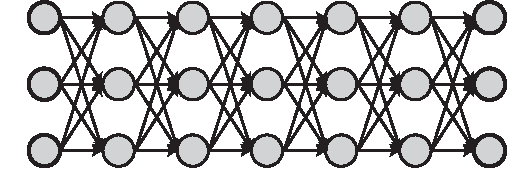
\includegraphics[scale=0.6]{figures/multiflow2.pdf}
	\caption{A ``layered''  graph for a multi-commodity flow problem.}
	\label{fig:multiflow}
\end{figure}
%
It consists of seven ``layers'' with three nodes each, and there are two commodities. From each node at a given level, there is a directed edge to each node at the next level. Sources are composed of the nodes at the first level, while the nodes at the last level constitutes the sinks. The capacity for each commodity and edge is 0 with a probability of 5\% and otherwise drawn from a uniform distribution between 5 and 15, while the common capacity of the edge e is 0 with probability 25\% and otherwise a number drawn from the uniform distribution between $s-10$ and $s$, where $s$ is the sum of the individual capacities on that edge. 

A multi-commodity flow problem is naturally block-structured with a block for each commodity, but it contains usually many global constraints, corresponding to the common upper limits for each edge. Therefore, instead of using these blocks to decompose the system, we divide the graph into smaller subgraphs, that is, for this particular graph we combine two layers into a block. We then treat the ingoing and outgoing edges in a subgraph as supply edges and demand edges, respectively, and eliminate all other variables than the corresponding supply and demand variables. Afterwards, the subgraphs are successively combined into larger graphs from which all but the corresponding supply and demand variables are eliminated. 

Similarly to Table~\ref{tab:projections}, Table~\ref{tab:multicom} shows the size of the original model and the projections resulting from a flat and decomposed projection, respectively. Both projections finished, and the projection time is also shown. Figure~\ref{fig:multicom} shows the progression over time of the number of inequalities and number of variables left to be projected, for both the flat and decomposed projection algorithm.

\begin{table}[b]
\caption{Size of projection of a multi-commodity flow model.}
\label{tab:multicom}
\centering
\btablesize
\begin{tabular}{l|r@{ / }r@{ / }r@{ / }r|r}
&\multicolumn{4}{c|}{Size}&\multicolumn{1}{c}{Time}\\
											&ineq (eq)&var &nzs &dens&\\
\hline
Original							&204 (42) & 120& 444&2.17&\multicolumn{1}{c}{-}\\
Presolved							& 59		  &  79& 201&3.41&\multicolumn{1}{c}{-}\\
Projected, decomposed	& 17 (2)  &  12&  61&3.59& 2h \phantom{9}9m \\
Projected, flat				& 17 (2)  &  12&  53&3.12& 17h 41m\\
\end{tabular}
\etablesize
\end{table}

Also here we see a reduction in the number of inequalities, variables and non-zero entries, of 3.5, 6.6, and 3.3/3.8 times, respectively (in both cases) compared to the presolved model. The density stays almost the same; for the decomposed model, the density increases with 5.3 \%, while the density decreases with 8.5\% for the flat projection.
This is not as big a reduction as for the VSMs, however, the unprojected models are also smaller to begin with. 
\begin{figure}[tb]
	\centering
		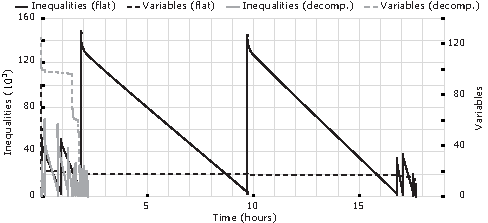
\includegraphics{figures/newMultiComGraph.pdf}
	\caption{Inequalities and variables during projection of a multi-commodity flow problem.}
	\label{fig:multicom}
\end{figure}

%%%%%%%%%%%%%%%%%%%%%%%%%%%%%%%%%%%%%%%%%%%%%%%%%%%%%%
\section{Related Work}
%\label{sec:related}
% Vi ska da også lige nævne vores eget
%Previous work has contributed frameworks for automated stowage planning (e.g., \cite{roach00,kimkang02,ambrosino04,low09,delgado09,pacino12}, and recently, linear stowage planning models were shown to scale to large container vessels (\cite{pacino11,AlbertosThesis}). These latter models embed an accurate capacity model, but since they specify the exact positions of the containers, they are too large for use as capacity models in uptake-, capacity-, fleet-, and network management, since these tasks often require several hundred capacity models to be solved simultaneously.  

Other FME-based frameworks for projection includes \cite{simon05,lukatskii08,shapot12}. 
Similar to our framework, these use simplifications, redundancy removal and approximation-procedures. For the latter, \cite{simon05} use the extreme-point method of \cite{huynh92}, while the boundary-approximation of \cite{lukatskii08,shapot12} involves a successive increase of the allowable deviation from the feasible area and a permissible maximal ratio of removed non-redundant inequalities.
Seen from the perspective of capacity models, both frameworks are used on quite small systems. Furthermore, the systems in \cite{simon} are also sparse. %The framework of \cite{simon05} is used on quite small and sparse systems, and the authors of \cite{lukatskii08,shapot12} performs tests with sizes between $81$ inequalities and $40$ variables to $201$ inequalities and $100$ variables.
%%These, however, only operate on what in our domain would be considered quite small systems. 
Our FME-based framework is to our knowledge the first that can take advantage of block-angular structure in the system.

%Particularly within linear programming, work has also been done in the area of classifying and removing redundant inequalities in a inequality system as well as finding implicit equalities, e.g. \cite{telgen83,lassez93,karwan83,andersen95,mattheiss73,brearley75,maros} to name a few. %de sidste to er nogen, vi har brugt og nævnt før
%Many of these are not applicable for us, since they eg. are to be performed within the simplex procedure or use an optimal extreme point. %However, we have used know methods for our preprocessing, eg. \cite{andersen95,brearley75,maros} in our preprocessing and clean-up method.

Other methods exist for computing the projection of a feasible area of an (in)equality system, that are not based on FME. The method in \cite{huynh92} finds extreme points in the projection space incrementally. It can therefore also be used to approximate the projection as is done in \cite{simon05}. It is recommended for dense systems. %Another method based on \cite{lassezlassez} is described in \cite{huynh92}, where the projection is computed by successive refinements of an initial approximation of the projection. According to the authors, the complexity of their algorithm ``depends essentially on the dimension of the projection of the output not the size of the input'' \cite{huynh92}, and could therefore be an interesting alternative to Fourier-Motzkin-elimination in a case like the one we consider. 
Another example is the method introduced in \cite{jones04}, which computes all facets of the projection iteratively using a face-lattice. 
This method is recommended by the authors for polytopes with a low facet count and a high vertex count.

\color{red}{Note: Jeg har skåret lidt fra om forskellen til de to frameworks. Jeg har slettet en ``anden metode til projection'', fordi jeg pludselig blev i tvivl om ikke det bare er det samme som den første, jeg nævner}
\color{black}
%%%%%%%%%%%%%%%%%%%%%%%%%%%%%%%%%%%%%%%%%%%%%%%%%%%%%%%%%%
\section{Conclusion}\label{sec:conclusion}
For a liner shipping company, accurate capacity models that succinctly represent the trade-off between the different types of containers are important in many areas such as uptake management, capacity management, network management, and fleet management. Although previous work on stowage models in principle provide fine-grained capacity models, they cannot readily be used in practice as such, since they are too large.
As an alternative, we have developed a framework based on Fourier-Motzkin elimination that automatically translates a linear stowage model (VSM) into a smaller sized capacity model (VCM) by projecting unneeded variables. The framework utilizes preprocessing, variable elimination (FME and Gauss-elimination), a parallel redundancy removal, as well as a boundary coarsening (removal of almost redundant inequalities). It uses a novel decompostion method that exploits the block-angular structure of the problem to speed up the projection.

Our results show that the projected VCMs are reduced by an order of magnitude both in number of inequalities and number of non-zero entries. The VCMs including hydrostatic constraints are solved 20-35 times faster than their corresponding VSMs, while the difference in objective value is 0.15-0.5 \%. For the models not including hydrostatic constraints, the speed-up is larger, but so is the loss of accuracy. The more realistic models including hydrostatic constraints are therefore more suited as submodels in optimization tasks within e.g. capacity management. 

Our framework makes use of a decomposition of the block-angular structure of the VSMs, and this decomposition drastically improves the runtime of the projections of the more complex stowage models. The block-angular structure is commonly found in real-world linear models, and our projection framework can be used for other problems. As an example, we have considered a multi-commodity flow problem and applied our framework. We found a similar speed-up as for the VSMs. 

There are several interesting directions for future work. 
From an application point of view, it could be interesting to test the VCMs in an actual setting for e.g. uptake management in a flow graph.
Likewise it could be interesting to  add more constraints to the VSM and/or investigate the limits for the decomposition framework. Of course, in this connection, various optimizations of the framework and its implementation, such as e.g. the mentioned parallellization of the projection of the subsystems of the decomposed system, would be useful to enhance the framework and further speed up the projection. Finally, for using the decomposition for different problems, it would be useful to have a procedure, that automatically estimates the best way of decomposing a given system. Finding and testing the framework on more block-angular problems in need of projection would also be of interest.

\subsection*{Acknowledgements}
We would like to thank Stefan R{\o}pke, Thomas Stidsen, and David Pisinger for discussions on applications of the FME framework beyond container vessel capacity models. This research is supported by the Danish Maritime Fund, Grant No. 2016-064.

\bibliographystyle{abbrv}
\bibliography{bibfile}
\end{document}
%%%%%%%%%%%%%%%%%%%%%%%%%%%%%%%%%%%%%%%%%%%%%%%%%%%%%%%%%%%%%%%%%%%%%%%%%%%%%%%%%%%%%%%%%%%%%%%%%%%
\appendix
%\scriptsize
%\section{Background} \label{sec:background}

%The cargo space of a container vessel is divided into parts called \textit{bays} that each consists of a grid of \emph{cells}. Each cell is divided into two \emph{slots} and can accordingly hold one standard $40'$ container or two $20'$ containers. Some cells have power plugs allowing for \emph{reefer} containers to be refrigerated as required. Each bay is divided into three or four parts called \textit{locations}, at which level the vessel's capacities are given. See Figure~\ref{fig:vessel}.

%\begin{figure}[tb]
%	\centering
%		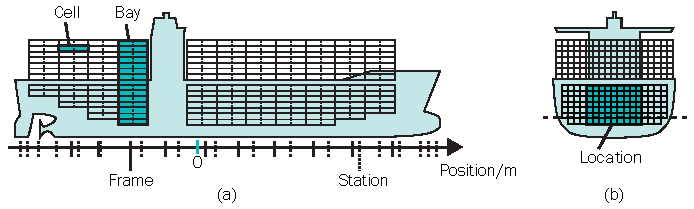
\includegraphics{figures/vessel3.pdf}
%	\caption{Vessel structure and reference points seen (a) on a longitudinal intersection and (b) on a transversal intersection.}
%	\label{fig:vessel}
%\end{figure}

%To define common reference points for cargo-holding structures and hydrostatic constraints, we further define larger \emph{sections} of the vessel and their endpoints. Each of these sections either span a number of succeeding bays, or a part of the ship containing no bays at all.
%See Figure~\ref{fig:sectionEndPoints}. Note that this is \emph{not} part of the data describing the vessel itself, but an input we define.
%
%\begin{figure}[tb]
%	\centering
%		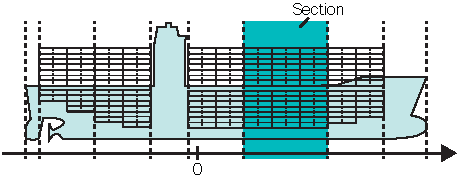
\includegraphics{figures/sectionEndPoints.pdf}
%	\caption{Sections on a vessel. Their endpoints are used as common reference points for cargo-holding structures and hydrostatic constraints in the VSMs.}
%	\label{fig:sectionEndPoints}
%\end{figure}
%
%An empty vessel without cargo, ballast or equipment is referred to as \emph{lightship}.  The lightship is given in the data by a set of ``blocks'' placed along the vessel. Each block has a given weight that is assumed to be uniformly distributed along the block.
%The cargo itself is described by a container \emph{type}, which is defined by a length ($20'$ or $40'$)\footnote{$45'$ long containers are also common, but for the sake of simplicity, we only consider $20'$ and $40'$ containers in this article.}, whether it is a reefer-container or not, and a weight class (in a discrete set of average weights). 
%Besides cargo bays, vessels also have \emph{ballast tanks} in fixed positions along the vessel that can be filled with water to improve the stability of the vessel.

%Though containers physically are placed in specific slots, the vessel data specifies capacities for each location. These capacities are given in \emph{TEU} (Twenty-foot Equivalent Units), i.e. a standard $20'$ container takes up one TEU, while a $40'$ container takes up two TEU. For each location, the vessel data includes upper bounds for: the total number of TEUs, $20'$ containers, $40'$ containers, reefer slots, reefer cells, plus separate total weight limit for $20'$ and $40'$ containers, respectively. The latter exist, since only $20'$ containers rest on the middle support posts of the stack it is in, while the end posts hold weight of both $20'$ and $40'$ containers. This may lead to different weight capacities of $20'$ and $40'$ containers. Limits for each ballast tank are likewise given in the input data, as well as a limit for the total displacement, i.e. the weight of the vessel, including ballast water, cargo and the ship itself. 

%On a vessel, stress forces arise as a result of gravitation acting downwards and buoyancy acting upwards. This results in shear forces and bending moments along the longitudinal axis of the vessel, and limits on these are given for a set of reference points along the vessel called \emph{frames} (see Figure~\ref{fig:vessel}(a)). The buoyancy force comes from the vessel's displacement of water and hence depends on the varying (and irregular) shape of the hull and the displacement of the vessel. The area submerged in water is given at another set of reference points called \emph{stations} for a discrete set of displacement values (see Figure~\ref{fig:vessel}(a)).
%The position of these reference points do not line up with bay endpoints, and this is remedied in the Vessel Stowage Model presented in the next section to allow for a less complex modelling. Further requirements to ensure the stability of the vessel are imposed in real life and considered e.g. in \cite{AlbertosThesis}, but are not included here.


%\section{Vessel Stowage Model (VSM)} \label{sec:stowmodel}
\scriptsize
This appendix presents the VSM used. %essel Stowage Model that is be projected to obtain the wanted Vessel Capacity Model (VCM). The model is adapted from work by Delgado (\cite{AlbertosThesis})/\ref{ICCL18}. %It relies on vessel data from a real vessel profile used by an industrial loading computer. The VSM includes various stowage constraints and further describes the hydrostatic constraints reasonably accurate while abstracting away much of the unnecessary complexity relating to the physical layout of the vessel that is present in the data. More specifically, the buoyancy data used in hydrostatic calculations are given at a set of points along the vessel (stations), while hydrostatic constraints are given in relation to another set of points (frames), and neither of these coincide with the position of the structures holding the cargo or the ballast tanks (see Figure~\ref{fig:vessel}(a)). The measure points are aligned in the VSM (see Figure~\ref{fig:sectionEndPoints}), and calculations for the hydrostatic constraints are simplified. 
%
The sets, variables and parameters used to describe the model are listed below. Buoyancy data and hydrostatic limits are translated to the sections' end points as explained in Section~\ref{sec:model}. %, and the derived parameters are included.

\begin{table}[tbp]
\begin{centering}
\scriptsize
\begin{tabular}{p{1.6cm}p{4.4cm}|@{\:}p{1.7cm}p{4.4cm}}
\multicolumn{2}{l}{\textbf{Sets}}\\
\hline\noalign{\smallskip}
$L$  																	& Locations. 												& $T$	 																	& Types of containers %(a length, weight, and reefer/non-reefer).
\\ 
$S$	 																	& Sections (ordered set).						& $T^{\{\trt{20},\trt{R}\}}\subseteq T$ & $20'$/reefer types, respectively. \\
$S^{\{\trt{f}, \trt{a}\}}\subseteq S$ & Sections fore/aft, respectively. 	& $\mi{BT}$ 														& Ballast tanks. \\
$L_s\subseteq L$ 											& Locations in section $s\in S$. 		& $F$	 																	& Frames.\\
$B$ 																	& Blocks with constant weight. 			& $\mi{ST}$ 														& Stations.\\
																			&																		& $D$																		& Displacement values.\\
\end{tabular}
\end{centering}
\end{table}

\begin{table}[tbp]
\scriptsize
\begin{tabular}{p{1.6cm}p{10.4cm}}
\multicolumn{2}{l}{\textbf{Variables}}\\
\hline\noalign{\smallskip}
$x_{l,\tau}\in \mathbb{R}^+_0$		& {Number of containers of type $\tau\in T$ to be stowed in location $l\in L$}.\\
$t_s\in \mathbb{R}^+_0$						& {The weight of ballast tanks within section $s\in S$.}\\
%\multicolumn{2}{l}{\textbf{Auxilliary variables}}\\
\hline\noalign{\smallskip}
$x_\tau\in \mathbb{R}^+_0$ 				& {The total number of containers of type $\tau\in T$.}\\
$w_s\in \mathbb{R}^+_0$						& {The total weight of section $s\in S$.}\\
$w\in \mathbb{R}^+_0$							& {The total displacement.}\\
$b_{s,d} \in\mathbb{R}^+_0$ 			& {The buoyancy force for section $s \in S$ with a total displacement of $d\in \mathbb{R}$.}\\
$\mi{sf}_s\in \mathbb{R}$ 				& {The shear force at the aft endpoint of section $s\in S$.}\\
$\mi{bm}_s\in \mathbb{R}$ 				& {The bending moment at the aft endpoint of section $s\in S$.}\\
\end{tabular}
\end{table}
\begin{table}[tb]
\scriptsize
\begin{tabular}{p{3.5cm}p{8.5cm}}
\multicolumn{2}{l}{\textbf{Parameters}}\\
\hline\noalign{\smallskip}
$C_l^{\{\trt{20}, \trt{40}, \trt{TEU}, \trt{RS}, \trt{RC}\}}\in \mathbb{N}$ 		
																														& Maximal capacity of  $20'$ containers, $40'$ container, TEUs, reefer slots, and reefer cells in location $l\in L$. \\
$C_l^{\{\trt{W20}, \trt{W40}\}}\in \mathbb{R}$							& {Weight capacity of  $20'$ and $40'$ containers in location $l\in L$.}\\
$W_{\{\tau,b\}}\in \mathbb{R}^+_0$													& {The weight of container type $\tau\in T$, and of block $b\in B$, respectively.} \\
$A_{\sigma, d}\in \mathbb{R}^+_0$ 													&	{The area submerged in water at station $\sigma\in ST$ for a displacement $d\in D$.}\\
$P^{\{\trt{f},\trt{a}\}}_{\{l,b,t\}}\in \mathbb{R}$ 				&	{The longitudinal position of the fore and aft endpoint of location $l\in L$, block $b \in B$, and tank $t \in BT$.}\\
$P_{f}$, $P_{\sigma}\in\mathbb{R}$ 
																														&	{The longitudinal position of frame $f \in F$, and of station $\sigma\in \mi{ST}$.}\\
$\mi{Max}^\trt{W}$, $\mi{Max}^\trt{WT}_b\in \mathbb{R}^+$		&	{Upper bound for the total displacement and for ballast tank $b\in BT$.}\\
$\mi{SF}^{\{+,-\}}_f$, $\mi{BM}^{\{+,-\}}_f\in\mathbb{R}$ 	&	{Upper/lower bounds for the shear force and bending moment at each frame $f\in F$.}\\
%\\
%\multicolumn{2}{l}{\textbf{Derived parameters}}\\
\hline\noalign{\smallskip}
$P^{\{\trt{f},\trt{a}\}}_s \in \mathbb{R}$ 									& {The fore and aft position of section $s \in S$.}\\  
$\mi{SF}^{\{+,-\}}_s$, $\mi{BM}^{\{+,-\}}_s\in\mathbb{R}$		& {Upper and lower bounds for the shear force and bending moment at the aft endpoint of section $s\in S$.}\\
$\mi{Max}^\trt{WT}_s\in \mathbb{R}$													& {Upper bound for the weight of ballast tanks in section $s\in S$.}\\
$A''_{p, d}\in \mathbb{R}^+_0$															&	{Approximation of the area submerged in water at a longitudinal position $p$ along the vessel for a displacement $d\in \mathbb{R}$.}\\
$\mi{PR}_{b,s}\in[0;1]$																			& {The percentage of the tank $b\in\mi{BT}$ that lies within section $s\in S$.}
\end{tabular}
\end{table}

 A container type $\tau \in T$ defines the container's length (20' or 40'), weight class (6, 21, or 27 tons), and whether it is a reefer or not. The set of stations, $ST$, includes $\sigma^\trt{a}$ and $\sigma^\trt{f}$, which are two (artificial) stations at the aft most and fore most positions of the ship, respectively. Similarly, $F$ contains the frames $f^\trt{a}$ and $f^\trt{f}$. The submerged areas for these stations and bounds for these frames are trivial. It is assumed that if $L_s\neq \emptyset$ then $L_s$ contains all locations that are positioned within some interval on the longitudinal axis. 

%The decision variables of the VSM are $x_{l,\tau}$ for all $l\in L$ and $\tau \in T$, denoting the number of containers of type $\tau$ stowed in location $l$, and $t_s$ for all $s\in S$, denoting the amount of ballast water in ballast tanks in section $s$. Even though $x_{l,\tau}$ is a number of containers and hence a natural number, we model it as a real number to ensure that the resulting model is a polyhedron. The auxiliary variables, $x_\tau$ for all $\tau\in T$ are the decision variables of the VCM. All other variables will be eliminated when we transform a VSM into its corresponding VCM. Hence, as required, a capacity model describes the free capacity trade-off between the different container types irrespective of where the containers are stowed on the vessel. The polyhedron representation of the 
The VSM is defined by the following linear equations. 
Equation \eqref{typeDef} defines the decision variables of the VCM. Equations \eqref{20Cap}-\eqref{reeferCellCap} defines the capacity constraints for each location.
%ensure that for each location of the vessel, the stowed containers are within the allowed capacities w.r.t. the number of $20'$ containers, $40'$ containers, TEUs, and the weight of the $20'$ and $40'$ containers, respectively.
%Likewise, equation \eqref{combinedWeightCap} ensures that the weight of a location is within limits, taken the different distribution of the weight of $40'$ containers, respectively $20'$ containers, within a slot into consideration. Equations \eqref{reeferSlotCap} and \eqref{reeferCellCap} ensure that there is enough reefer plugs for reefer containers. 
\eqref{totalWeightDef} and \eqref{totalDisp} defines the weight of each section and the total displacement, respectively, and \eqref{btLim} and \eqref{wTotalLim} limits (defines capacity of) the ballast weight in each section and the total displacement, respectively.
The hydrostaic forces and moments are defined in \eqref{defBancy}-\eqref{bmA}, while \eqref{sfLim} and \eqref{bmLim} limits them.
Finally, \eqref{xPos} requires the decision-variables to be non-negative.
\begin{align}
	\label{typeDef}
	&x_\tau = \sum_{l\in L} x_{l,\tau} 
			&& \forall{\tau \in T}.\\
	%
		\label{20Cap}
	&\smashoperator[r]{\sum_{\tau \in T^\trt{20}}} x_{l,\tau} \leq C_l^\trt{20}
			&& \forall l \in L.\\
	%
	\label{40Cap}    	
	&\smashoperator[r]{\sum_{\tau \in T\setminus T^\trt{20}}} 2\cdot x_{l,\tau} \leq C_l^\trt{40} 
			&& \forall l \in L.\\
	%
	\label{teuCap}
	&\smashoperator[r]{\sum_{\tau \in T^\trt{20}}} x_{l,\tau} + 2\cdot\smashoperator[lr]{\sum_{\tau \in T\setminus T^\trt{20}}} x_{l,\tau} \leq C_l^\trt{TEU} 
			&& \forall l \in L.\\
	%
	\label{weight20Cap}
	&\smashoperator[r]{\sum_{\tau \in T^\trt{20}}} W_\tau\cdot x_{l,\tau} \leq C_l^\trt{W20} 
			&& \forall l \in L.\\
	%
%	\label{weight40Cap}
%	&\smashoperator[r]{\sum_{\tau \in T\setminus T^\trt{20}}} W_\tau\cdot x_{l,\tau} \leq C_l^\trt{W40} 
%			&& \forall l \in L. \\
	%
	\label{combinedWeightCap}
	&0.5 \smashoperator[lr]{\sum_{\tau \in T^\trt{20}}} W_\tau\cdot x_{l,\tau} + \smashoperator[lr]{\sum_{\tau \in T\setminus \in T^\trt{20}}} W_\tau\cdot x_{l,\tau} \leq C_l^\trt{W40} 
			&& \forall l \in L.\\
	%
	\label{reeferSlotCap}
	&\smashoperator[r]{\sum_{\tau \in T^\trt{R}}} x_{l,\tau} \leq C_l^\trt{RS} 
			&& \forall l \in L. \\
	%
	\label{reeferCellCap}
	&\smashoperator[lr]{\sum_{\tau \in T^\trt{R}\cap T^\trt{20}}} 0.5\cdot x_{l,\tau} + \smashoperator[lr]{\sum_{\tau \in T^\trt{R}\setminus T^\trt{20}}} x_{l,\tau} \leq C_l^\trt{RC} 
			&& \forall l \in L.\\
	%
	\label{totalWeightDef}
	&w_s = \sum_{\tau \in T} \sum_{l\in L_s} W_\tau\, x_{l,\tau} + xt_s + \sum_{b\in B} \mi{PR}_{b,s}\cdot W_b 
			&& \forall s \in S.\\
	%
	\label{totalDisp}
	&w  = \sum_{s\in S} w_s. 
			&&\\
	%
	\label{btLim}
	&0 \leq t_s \leq \sum_{b \in BT} \mi{PR}_{b,s}\cdot \mi{Max}^\trt{WT}_b 
			&& \forall s\in S.\\
	%
	\label{wTotalLim}
	&w \leq \mi{Max}^\trt{W}. 
			&&\\
	%
	\label{defBancy}
	&b_{s,d} = \smashoperator[lr]{\sum_{p \in Q\setminus \{P^\trt{f}_s\}}} 0.5\cdot(A''_{p,d}+A''_{\mi{next}_p,d})\cdot (\mi{next}_p-p), 
			&& \forall s\in S, d\in \mathbb{R}.\\%\text{where } \mi{next}_p = \min\set{p' \in P}{p' > p}.\\
	%
	\label{sfF}
	&\mi{sf}_s = \smashoperator[r]{\sum_{s' \in S. P^\texttt{f}_{s'} \geq P^\texttt{f}_s}} (w_{s'} - b_{s',w}) 
			&& \forall s \in S^\texttt{f}.\\
	%
	\label{sfA}
	&\mi{sf}_s = \smashoperator[r]{\sum_{s' \in S. P^\texttt{a}_{s'} < P^\texttt{a}_s}} (w_{s'} - b_{s',w}) 
			&& \forall s \in S^\texttt{a}.\\
	%
	\label{bmF}
	&\mi{bm}_s = 	\smashoperator[r]{\sum_{s' \in S. P^\texttt{f}_{s'} \geq P^\texttt{f}_s}} (w_{s'} + b_{s',w})\cdot |P^\trt{a}_s - \frac{P^\trt{f}_{s'}-P^\trt{a}_{s'}}{2}|
			&& \forall s \in S^\texttt{f}.\\
	%
	\label{bmA}
	&\mi{bm}_s = \smashoperator[r]{\sum_{s' \in S. P^\texttt{a}_{s'} < P^\texttt{a}_s}} (w_{s'} + b_{s',w})\cdot |P^\trt{a}_s - \frac{P^\trt{f}_{s'}-P^\trt{a}_{s'}}{2}|
			&& \forall s \in S^\texttt{a}.\\
	%
	\label{sfLim}
	&\mi{SF}^-_s \leq \mi{sf}_s \leq \mi{SF}^+_s
			&& \forall s \in S.\\
	%
	\label{bmLim}
	&\mi{BM}^-_s \leq \mi{bm}_s \leq \mi{BM}^+_s 
			&& \forall s \in S. \\
	%
	\label{xPos}
	& 0\leq x_{l,\tau}, t_s   
			&& \forall l\in L, \tau\in T, s\in S.
\end{align}

\end{document}
	
For defining the weight of a section, we need its fore and aft position. For \emph{cargo-containing sections}, i.e. sections $s$ for which $L_s\neq \emptyset$, we can find immediate fore- and aft points of the locations in $s$: $P^\trt{if}_s = \max\set{P^\trt{f}_l}{l\in L_s}$, and $P^\trt{ia}_s = \min\set{P^\trt{a}_l}{l\in L_s}$ (see Figure~\ref{fig:sections}). There is a small gap between two consecutive bays, and this space is divided evenly between two consecutive, cargo-containing sections. Sections that are not cargo-containing get their endpoints from the immediate end points of their neighbor sections if these are cargo-containing, and otherwise the non-cargo-containing parts of the vessel is divided evenly among the corresponding non-cargo-containing sections. See Figure~\ref{fig:sections}.
%\begin{figure}[tb]
%	\centering
%		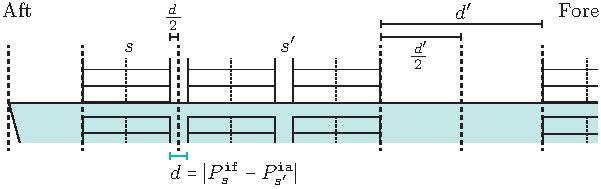
\includegraphics{figures/sections.pdf}
%	\caption{The doted lines indicates the endpoints of the sections.}
%	\label{fig:sections}
%\end{figure}
Using the end points of the sections, equation \eqref{totalWeightDef} defines the total weight of section $s\in S$, including cargo, ballast tanks and the vessel itself. Equation \eqref{totalDisp} defines the total displacement (weight) of the vessel.  Here, $\mi{PR}_{b,s}$ defines the percentage of tank $b$ that lies within section $s\in S$, that is 
\[
\mi{PR}_{b,s} = \frac{\max(\min(P^\texttt{f}_b, P^\texttt{f}_s)-\max(P^\texttt{a}_b, P^\texttt{a}_s),0)}{P^\texttt{a}_s-P^\texttt{f}_s}.
\]

Capacities for individual tanks are pooled into capacities for tanks within a section, such that the amount of ballast water in any section $s$ is limited by the amount of water in the portion of each tank that lies within that section combined, and further it is required to be non-negative \eqref{btLim}. Likewise, the number of containers of each type placed in each section is non-negative \eqref{xPos}. Finally, the total displacement (weight) is required to be within limits \eqref{wTotalLim}.

For a station $\sigma\in\mi{ST}$, the submerged area of the cross-section for a given displacement $d\in D$ is given by $A_{\sigma,d}$. From these values we make an approximation of the submerged area at $\sigma$ for any positive displacement $d\in \mathbb{R}_o^+$. This is done by linearizing the values between the maximal displacement value given in the table, $d_\mi{max}=\text{max}\{d\in D\}$, and a displacement value $d_\mi{min}$ at the point, where the hull does not curve too much anymore. For the cross-section given in Figure~\ref{fig:vessel}(b) this would correspond to the displacement giving rise to the marked waterline. We note that since our VSM will mainly be used for some sort of maximization of loaded cargo it is fair to assume that the displacement will be above the found $d_\mi{min}$. Thus, the approximation of the submerged area is  
\[
A'_{\sigma,d} = \frac{A_{\sigma,d_{max}} - A_{\sigma,d_{min}}}{d_{max} - d_{min}} \cdot (\mi{w} - d_{max}) + A_{\sigma,d_{max}} \quad \forall d\in \mathbb{R}^+_0.
\]
The submerged area between two consecutive stations $\sigma$ and $\sigma'$ are then linearized, so that the submerged area for displacement $d$ at any point $p\in[P_\sigma;P_{\sigma'}]$ is approximated by
\[
A''_{p,d} = \frac{A'_{\sigma',d}-A'_{\sigma,d}}{P_{\sigma'}-P_\sigma}\cdot(p-P_\sigma) + A'_{\sigma,d}.
\]
From this an approximation of the buoyancy of section $s\in S$ for a given $d\in \mathbb{R}^+_0$ is calculated by averaging the areas between the two endpoints of $s$ and multiplying with the distance between the points and the density of salt water.\footnote{Though all weights in principle have to be multiplied by the gravitational acceleration to get a force, it is a common practice to omit this in these calculations.} If there are stations lying within $s$, several volumes are calculated and added. Thus, let $Q_s := \{P^\trt{a}_s, P^\trt{f}_s\} \cup \set{P_\sigma}{\sigma\in ST,\; P^\trt{a}_s < P_\sigma < P^\trt{f}_s}$ be the section's end points together with the stations between the two endpoints, and let $\mi{next}_p = \min\set{p' \in Q_s}{p' > p}$ be the next point in $Q$ (in the direction of the bow) for each $p \in Q_s\setminus \{P^\trt{f}_s\}$. Then the buoyancy of section $s\in S$ at a displacement $d\in\mathbb{R}^+_0$ is defined by equation \eqref{defBancy}. 

To obtain upper (lower) bounds for the shear force at the sections' aft endpoints,  we linearize the upper (lower) bound for the shear force between two consecutive frames as a function of their position. To obtain the bounds for the shear force at the aft endpoint of $s$, we then use this linearization given by the point's two closest surrounding frames. Similarly for the upper and lower bounds for the bending moment. Thus, the upper bounds for the shear force at the aft endpoint of section $s\in S$ is
\[
\mi{SF}^+_s = \frac{\mi{SF}^+_{f_2}-\mi{SF}^+_{f_1}}{P_{f_2}-P_{f_1}}\cdot(P^\trt{a}_s - P_{f_1}) + \mi{SF}^+_{f_1}, 
\]
where $f_1 = \text{argmax}_{\set{f\in F}{P_f\leq P^\trt{a}_s}}P_f$ and $f_2 = \text{argmin}_{\set{f\in F}{P_f>P^\trt{a}_s}}P_f$. Of course, if there is an $f\in F$ such that $P^\trt{a}_s = P_f$ then we let $\mi{SF}^+_s = \mi{SF}^+_f$. Similarly we find $\mi{SF}^-_s$, as well as $\mi{BM}^+_s$ and $\mi{BM}^\trt{-}_s$. Given a displacement $d\in\mathbb{R}^+_0$, the shear forces and bending moment at each section $s$'s aft endpoint can then be calculated. If $s\in S^\trt{f}$ ($s\in S^\trt{a}$), then the shear force at the aft endpoint equals the total weight $w_s$ of the sections fore (aft) $P^\trt{a}_s$ minus the buoyancy of the sections fore (aft) $P^\trt{a}_s$. Similarly, the bending moment at section $s$'s aft endpoint is calculated as the sum of resulting forces of sections $s'$ lying fore (aft) $P^\trt{a}_s$ times the distance from $P^\trt{a}_s$ to $s'$'s (longitudinal) midpoint. Equations \eqref{sfF} - \eqref{bmLim} define these shear forces and bending moments and require them to be within the found limits.
\end{document}
\section{Related Work}
\label{sec:preWork}
Previous work on stowage planning optimization (e.g., \cite{roach00,kimkang02,ambrosino04,low09,delgado09,pacino12}) has contributed frameworks for automated stowage planning, and recently, linear stowage planning models were shown to scale to large container vessels (\cite{pacino11,AlbertosThesis}). Since these models define the set of legal stowage conditions, they can be used to compute the residual capacity of a container vessel as a result of the interaction between the different types of containers to load. In other words, they embed an accurate capacity model. 

However, the use of these stowage models as capacity models is limited due to their size. Since a stowage model not only models the capacity of a vessel as a function of the different container types to load but also describes the position of the containers on the vessel, it may contain tens of thousands of constraints and variables and take long time to solve. This is a problem if the stowage model is to be used as a capacity model in uptake-, capacity-, fleet-, and network management, since these tasks often require several hundred capacity models to be solved simultaneously. For example, the task in uptake management of maximizing uptake over a set of voyages, requires us to associate a capacity model with each individual leg of the voyages and then optimize the resulting model.  

Our FME-based framework for variable elimination is to our knowledge the first that can take advantage of block-angular structure in the system. In \cite{simon05} Simon and King combine FME, Gauss-elimination, removal of linearly dependent inequalities and complete redundancy removal in a similar fashion as we have done, to project sparse systems. Moreover, they use the extreme point method of Huynh \textit{et al.} \cite{huynh92} to make approximations of the projection when this is necessary. Their method is implemented as part of an argument-size analyzer for logic programs and tested on a variety of these. Their elimination procedure is therefore not applied once, but instead multiple times during an analysis, and their method and results are for that reason hard to compare to ours. The (in)equality systems operated on are rather sparse and quite small, while their objective is to do the analysis more efficiently (faster) than other methods (when using the polyhedral abstract domain for program analysis). 

Lukatskii and Shapot \cite{lukatskii08}, \cite{shapot12} describe and implement a projection method using FME augmented with \v{C}ernikov's rules. They further use techniques for full redundancy removal examining the solution matrix for a basic solution. Further, they present and apply a method for ``additional matrix clean up'', where some almost redundant inequalities are removed. Their method for this is a little more elaborate than ours and involves a successive increase of the allowable deviation (corresponding to our $\epsilon$) and a permissible maximal ratio between the number of inequalities in the current system compared to the original system. They perform tests on a prototype implementation, where the size ranges between $81$ inequalities and $40$ variables to $201$ inequalities and $100$ variables, i.e., the systems they project are much smaller than the ones we have considered; granted, their run time is also smaller than ours. 

Separately, particularly within linear programming, work has also been done in the area of classifying and removing redundant inequalities in a inequality system as well as finding implicit equalities, e.g. \cite{telgen83}, \cite{lassez93}, \cite{karwan83}, \cite{andersen95}, \cite{mattheiss73} to name a few. 
Many of these (e.g. \cite{telgen83} and the {majority} of the methods presented in \cite{karwan83}) are to be performed within the simplex procedure (used to optimize an LP) or use the objective function and/or the optimal extreme point for the LP, and are hence not applicable for us. On the other hand, we have used cheap redundancy-identifications e.g. described in \cite{andersen95}, \cite{brearley75} and \cite{maros} in our preprocessing and clean-up method, as well as the removal of linearly dependent inequalities from \cite{lassez93}.

Other methods exist for computing the projection of a feasible area of an (in)equality system, that are not based on FME. For example, in \cite{huynh92}, the authors describe a method (based on a method from \cite{lassez90}) that they recommend for dense systems, called the extreme point method. The method works by finding the extreme points of the polytope $P$ defined by the convex combinations of constraints in $S$ that eliminate the variables in $Y$. Since the method finds extreme points and hence inequalities in the projection space incrementally, the method can be used to approximate the projection. The method is consequently used as a supplement to FME, Gauss elimination and full redundancy removal in \cite{simon05}, when the system being projected becomes too dense and an approximation is required.

Huynh, Lassez and Lassez \cite{huynh92} further describe a method (based on \cite{lassezlassez}), the convex hull method, in which the projection of an inequality system $S$ is computed by successive refinements of an initial approximation of the projection. According to the authors, the complexity of their algorithm ``depends essentially on the dimension of the projection of the output not the size of the input'' \cite{huynh92}, and could therefore be an interesting alternative to Fourier-Motzkin-elimination in a case like the one we consider. Another example is the method introduced in \cite{jones04}, called equality set projection, which computes all facets of the projection by first finding a random facet and then iteratively computing all adjacent facets (without revisiting them) {using a face-lattice}. 
This method is recommended by the authors for polytopes with a low facet count and a high vertex count.
\end{document}
